\section{Simulation study}
\label{sec:sim}
In this section, a simulation study is reported to compare the performance of OMERF with that of similar classification methods on various simulated datasets.
In Section \ref{sec:simdesign} it is described the design of the created datasets, while in Section \ref{sec:simres} the results are analysed, in order to assess advantages and drawbacks of OMERF.

\subsection{Simulation design}
\label{sec:simdesign}
With the aim of generating ordered categorical data, the R package \(simstudy\) \cite{simstudy} is used and in particular the function \(genOrdCat\).
This function uses an underlying (continuous) latent process \(w\) as the basis for data generation.
Assuming that probabilities are determined by segments of a logistic distribution, it defines the ordinal mechanism
using thresholds along the support of the distribution. For example, in case of \(k\) possible responses, then there will be \(k-1\) thresholds.
The area under the logistic density curve of each of the regions defined by those thresholds (there will be \(k\)
distinct regions) represents the probability of each possible response tied to that region.
In the simulation study we set \(k\) = 3 and the underlying latent process is generated as:
\begin{equation}
    \label{eq:simstudy1}
    \begin{aligned}
        w=f(\bm{x}_{ij}) + \sum_{q=0}^{Q} z_{qij}^T b_{qi} \qquad j=1,\dots,n_{i} \qquad i&=1,\dots,I \qquad c=1,\dots,C-1
    \end{aligned}
\end{equation}
where \(f\) is the fixed effects functional form which takes in input the \(p\)-dimensional vector of fixed effects covariates and \(\sum_{q=0}^{Q} z_{qij}^T b_{qi}\) are the random effects.

Regarding the fixed effects part we use a variation of the simulation design proposed in \cite{pellagatti2021generalized}.
The design for \(f\) incorporates both a linear component and a tree-like component, along with interactions among the covariates.
This approach allows to simulate a scenario with a highly diverse structure, which will challenge the flexibility and adaptability of our method.

Specifically, seven covariates are taken into account and \(f\) is modelled as follows:
\begin{equation}
    \label{eq:simstudy2}
    \begin{aligned}
        f(x_{1}, \dots,x_{7}) = \alpha(3+7x_{1}^2-5x_{2}+x_{2}x_{3}^2) + \beta tree(x_{4},x_{5},x_{6})
    \end{aligned}
\end{equation}

Here, \(\alpha\) and \(\beta\) represent two design parameters employed to regulate the importance given to the linear and tree-based part in the various Data Generating Processes (DGPs) for the simulation study.
The function \(tree(x_{4}, x_{5}, x_{6})\) follows the tree like stucture outlined in Figure \ref{fig:tree}.
The variable \(x_{7}\) is included even though it is not significant, in order to assess whether the algorithm is influenced by it. Indeed, while all of the seven covariates are
being used as predictors in the compared models, only the first six of them are actually used to generate \(f\).

The seven covariates are generated randomly in accordance with the following distributions:
\(X_{1},X_{2},X_{3}\sim N(0,1); X_{4}\sim U(-3,3); X_{5}\sim U(-6,6); X_{6}\sim U(-5,5); X_{7}\sim U(-4,4)\).

\begin{figure}[H]
    \centering
    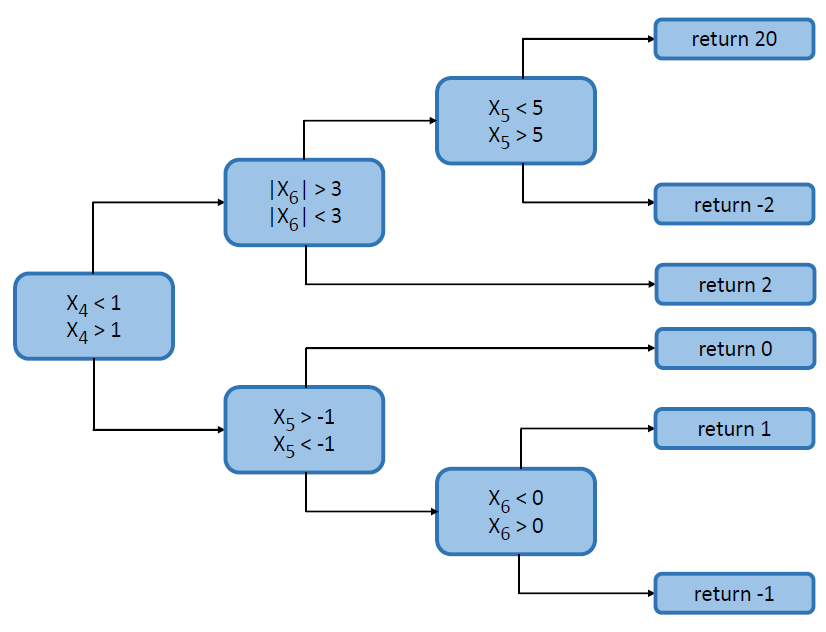
\includegraphics[width=0.5\textwidth]{tree_structure.png}
    \caption{Tree-like structure \(tree(x_{4},x_{5},x_{6})\) of the fixed effects part in Equation \refeq{eq:simstudy2}.}
    \label{fig:tree}
\end{figure}

The random effects are drawn from a normal distribution for two distinct scenarios:
\begin{itemize}
    \item \(Random \quad intercept \quad only: \sum_{q=0}^{Q} z_{qij}^T b_{qi} = b_{0i} \sim \mathcal{N}(0, \sigma^2_1)\), where \(\sigma^2_1\) is a design parameter which gives the possibility to change the variability of the effects in the different simulations.
    Indeed, within each scenario, two specifications (low and high) for the parameter \(\sigma^2_1\) are considered in order to account for different levels of magnitude of the between-group variability;
    \item \(Random \quad intercept \quad and \quad slope: \sum_{q=0}^{Q} z_{qij}^T b_{qi} = b_{0i} + x_{1ij}^T b_{1i}\), where \(x_{1ij}\) is the first fixed effects covariate and the random coefficient is \(\bm{b}_i \sim \mathcal{N}_2(0, \Sigma)\), with \(\Sigma=diag(\sigma^2_1;\sigma^2_2)\).
    It is important to note that the random effects \(b_{0i}\) and \(b_{1i}\) are treated as independent for any given value of \(i\), and as in the previous scenario \(\sigma^2_1\) and \(\sigma^2_2\) serves as parameters that regulates the random effects variance.
    In this setting, the covariate \(x_1\) is not assumed to have a fixed effect that applies uniformly across all observations. Instead, its impact is considered group-specific, meaning that \(x_1\) is assumed to have different effects across observations belonging to distinct groups.
\end{itemize}

In particular, a two-level data structure of \(I = 10\) groups with \(n_{i} = 100\) observations each is simulated, for a total number of units equal to 1000.
Note that for simplicity, an equal number of observations for each group is taken to ensure a balanced dataset. However, the model is, of course, capable of handling datasets with varying group sizes.

In addition to this simulation design approach, a more linear DGP is implemented in order to observe how OMERF method performs in a simpler context. In this case the first three covariates generated before are combined as follows:
\begin{equation}
    \label{eq:simstudy3}
    \begin{aligned}
        f(x_{1}, \dots,x_{3}) = 3+7x_{1}-5x_{2}+x_{2}x_{3}.
    \end{aligned}
\end{equation}
Only the case of a single, normally distributed random intercept is considered: \(b_{0i} \sim \mathcal{N}(0, \sigma^2_1)\).

All the design parameters listed before are chosen in order to obtain balanced simulated datasets regarding the classes of the ordinal response.
Moreover, several combinations of parameters are tested to observe how the model reacts in the case of a more polynomial or more tree-like response and with the variance related to random effects being higher or lower.
Thus, a total of 10 DGPs summarised in Table \ref{table:DGPs} are obtained. The main objective of the designed DGPs is to show how our algorithm is able to capture the variability of the groups and the nonlinear relationships of the data structure.
With these DGPs the OMERF's performance is evaluated in comparison to other three models: 
\begin{itemize}
    \item CLM and CLMM, from the \(ordinal\) R package \cite{ordinal}, which are expected to perform well in a linear context but are not able to model more complex structures, and in the case of CLM not even to grasp the hierarchical structure of data;
    \item Ordinal random forest, from the \(ordinalForest\) R package \cite{hornung2020ordinal}, which, as typical of ensemble tree-based models, is able to capture nonlinear relationships, but can not catch the nested structure.
\end{itemize}
These methods are chosen in order to, at least to some extent, include a range of both cumulative link and tree-based models.

\begin{table}[H]
    \centering 
    \begin{tabular}{|p{4em} | c | c | c | c | c |}
    \hline
    \rowcolor{bluePoli!40}
    & \textbf{\(f(\bm{x}_{ij})\)} & \textbf{\(\alpha\)} & \textbf{\(\beta\)} & \textbf{\(\sigma^2_1\)} & \textbf{\(\sigma^2_2\)} \T\B \\
    \hline \hline
    \textbf{DGP 1} & \(\alpha(3+7x_{1}^2-5x_{2}+x_{2}x_{3}^2) + \beta tree(x_{4},x_{5},x_{6})\) & 0.3 & 0.7 & 1 & - \T\B \\
    \textbf{DGP 2} & \(\alpha(3+7x_{1}^2-5x_{2}+x_{2}x_{3}^2) + \beta tree(x_{4},x_{5},x_{6})\) & 0.7 & 0.3 & 1 & - \T\B \\
    \textbf{DGP 3} & \(\alpha(3+7x_{1}^2-5x_{2}+x_{2}x_{3}^2) + \beta tree(x_{4},x_{5},x_{6})\) & 0.3 & 0.7 & 5 & - \T\B \\
    \textbf{DGP 4} & \(\alpha(3+7x_{1}^2-5x_{2}+x_{2}x_{3}^2) + \beta tree(x_{4},x_{5},x_{6})\) & 0.7 & 0.3 & 5 & - \T\B \\
    \textbf{DGP 5} & \(\alpha(3+7x_{1}^2-5x_{2}+x_{2}x_{3}^2) + \beta tree(x_{4},x_{5},x_{6})\) & 0.3 & 0.7 & 0.3 & 0.5 \T\B \\
    \textbf{DGP 6} & \(\alpha(3+7x_{1}^2-5x_{2}+x_{2}x_{3}^2) + \beta tree(x_{4},x_{5},x_{6})\) & 0.7 & 0.3 & 0.3 & 0.5 \T\B \\
    \textbf{DGP 7} & \(\alpha(3+7x_{1}^2-5x_{2}+x_{2}x_{3}^2) + \beta tree(x_{4},x_{5},x_{6})\) & 0.3 & 0.7 & 1 & 1 \T\B \\
    \textbf{DGP 8} & \(\alpha(3+7x_{1}^2-5x_{2}+x_{2}x_{3}^2) + \beta tree(x_{4},x_{5},x_{6})\) & 0.7 & 0.3 & 1 & 1 \T\B \\
    \textbf{DGP 9} & \(3+7x_{1}-5x_{2}+x_{2}x_{3}\) & - & - & 1 & - \T\B \\
    \textbf{DGP 10} & \(3+7x_{1}-5x_{2}+x_{2}x_{3}\) & - & - & 5 & - \B \\
    \hline
    \end{tabular}
    \\[10pt]
    \caption{Simulation parameters of both fixed and random effects parts for 10 different DGPs.}
    \label{table:DGPs}
\end{table}

\subsection{Simulation results}
\label{sec:simres}
For each of the ten DGPs described in Table \ref{table:DGPs} we simulate the dataset 100 times with 1000 observations each. In order to evaluate the predictive performances of the four compared models, each dataset is randomly split into training and test sets, with a ratio of 80\% for training and 20\% for testing.
To evaluate the quality of the predictions the five performance measures presented in Section \ref{sec:gof} are computed. Simulation results, consisting of mean and variance of each set of simulations for each index,  are reported in Tables \ref{table:res_int}, \ref{table:res_slope} and \ref{table:res_lin}.

From the findings reported in these tables, it can be inferred that generally, all performance measures in each simulation are consistent in the results. In particular, the performance of the created OMERF method is always good, and, even when not the best, remains mostly comparable to that of the top-performing model.

Note that the difference in effectiveness between tree-based methods (ordianl forest and OMERF) and linear models (CLM and CLMM) is especially significant when the DGP has a more tree-like structure (e.g. DGPs 1,3 in Table \ref{table:res_int}).
On the other hand, in cases where the DGP is based on a more polynomial structure (e.g. GDPs 2,4 in Table \ref{table:res_int}), the ordinal random forest and OMERF models still better capture the complexity of the problem, but the difference with the basic linear models is more negligible.
Indeed, the OMERF method reaches the best performance in DGP 2 (with \(Accuracy\) = 0.8039, \(MSE\) = 0.2646, \(ARI\) = 0.5324, \(Cohen's \, k\) = 0.5092, \(Cardoso \, idx\) = 0.2918, \(Ballante \, idx\) = 0.0960),
but has the largest difference in performance compared to the linear models in DGP 1, with an accuracy 0.0784 higher than CLM and 0.08 higher than CLMM.

Even with the introduction of a random slope (namely in the cases reported in Table \ref{table:res_slope}), the models' performance remains consistent with those analysed so far.
Moreover, in all the simulations there appear to be no major differences between the cases with small or large variability fixed effects.

On the contary, in DGPs 9 and 10 in Table \ref{table:res_lin}, which are specifically constructed with linear relationships, it is evident that CLM and CLMM tend to perform better with respect to the other models.
This result confirm that tree-based methods better capture nonlinear dependencies, but when there are linear data structures, simpler models are preferable, additionally yielding results that are usually more easily interpretable.

As for the variances in the estimations, all models estimates present small variability. Indeed, even OMERF is able to provide stable estimates, probably due to the iterative nature of the algorithm, which stabilizes the results.

Finally, since OMERF alternates between a random forest and a CLMM model, it takes the advantages of both methods.
Indeed, reporting in Figures \ref{fig:ranefDGP1} and \ref{fig:fix_cov_DGP1} the results in one of the runs of DGP 1 as a reference, it is evident how it succesfully manages to capture both the nested structure of the 10 random groups thanks to the CLMM, and the nonlinear relationships between the target value and the covariates, thanks to the RF.

\begin{figure}[H]
    \centering
    \subfloat[Original random coefficients taken from the normal distribution \(\sim \mathcal{N}(0, 1)\), as described in the simulation design in Section \ref{sec:simdesign}.\label{fig:original_re}]{
        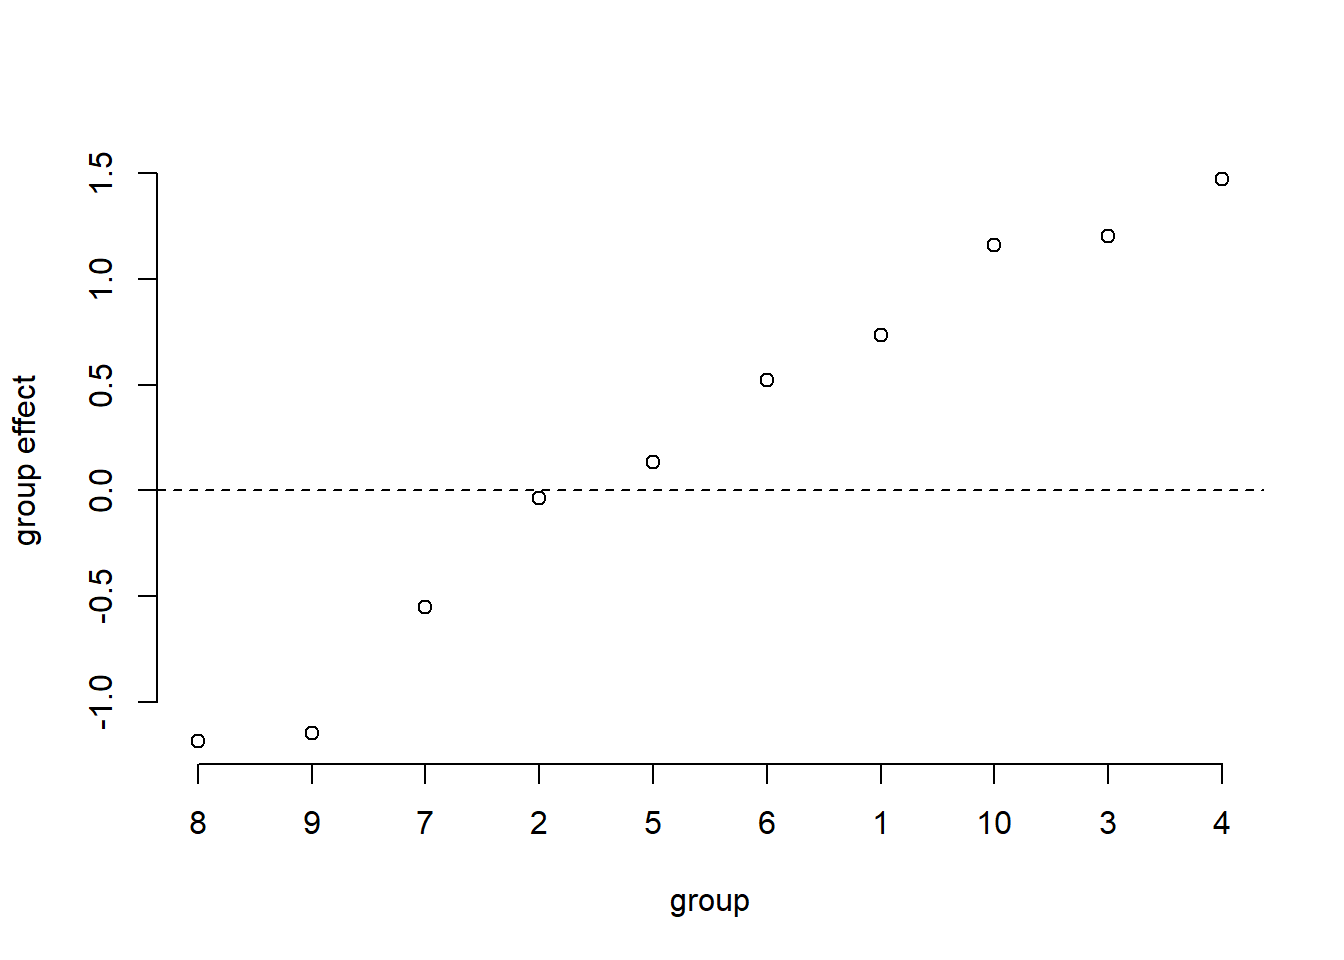
\includegraphics[scale=0.4]{Images/ranef1.png}
    }
    \quad
    \subfloat[Random intercepts with their confidence intervals, relative to the 10 simulated groups estimated by the OMERF method.\label{fig:estim_re}]{
        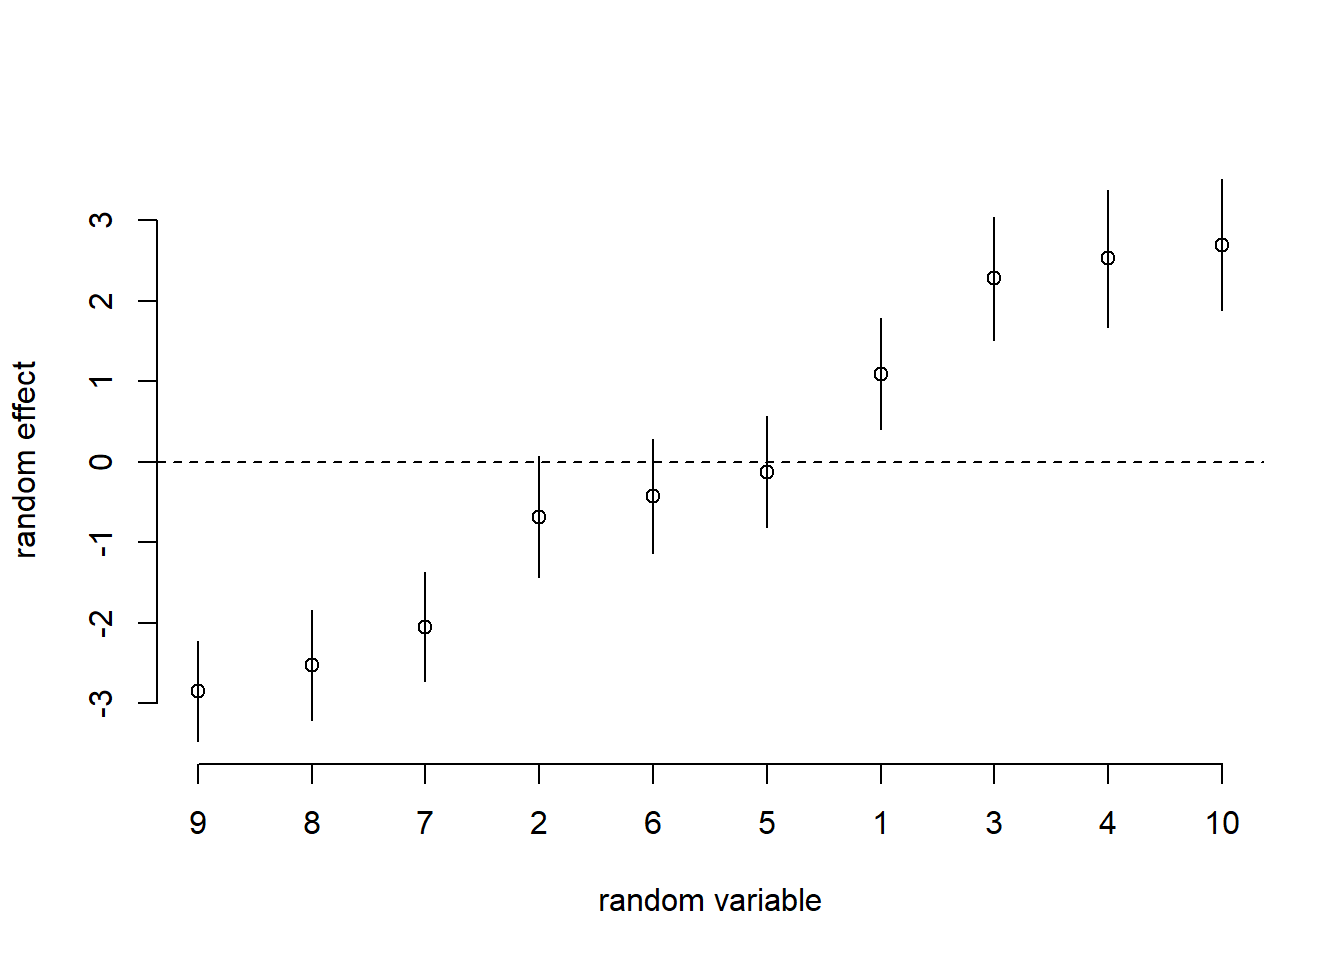
\includegraphics[scale=0.4]{Images/ranef2.png}
    }
    \caption[]{Random effects in one of the runs of DGP 1, listed in Table \ref{table:DGPs}.}
    \label{fig:ranefDGP1}
\end{figure}


\begin{figure}[H]
    \centering
    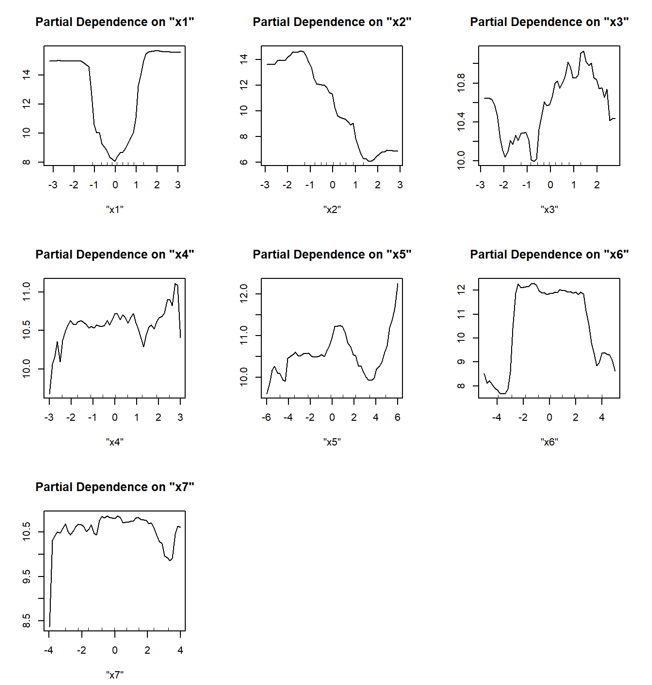
\includegraphics[width=0.8\textwidth]{fix_cov_sim.png}
    \caption{Partial plots of the random forest target value in the OMERF method with respect to the seven covariates of DGP 1, described in Table \ref{table:DGPs}. The \(y\)-axis reports the increment/decrement of the target value, given the covariate on the \(x\)-axis.}
    \label{fig:fix_cov_DGP1}
\end{figure}

Figure \ref{fig:ranefDGP1} recreates the differences in the hierarchical level (Figure \ref{fig:estim_re}) comapred to the original random coefficients taken from the normal distribution (Figure \ref{fig:original_re}).
Figure \ref{fig:fix_cov_DGP1} shows, on the other hand, the association of covariates and response, giving an insight into the underlying latent process behind the ordinal model. It can be observed that the algorithm captures the quadratic and inverse linear trend in the variables \(x_1\) and \(x_2\) respectively.

In conclusion, in a nonlinear setting the proposed method performs better with respect to CLM and CLMM, and comparably to ordinal random forest; having the advantage of increasing the knowledge about the multilevel nature of data.

\begin{table}[H]
    \centering 
    \begin{tabular}{|p{4em} c c c c c c c |}
    \hline
    \rowcolor{bluePoli!40}
    & \textbf{Model} & \textbf{Acc} & \textbf{MSE} & \textbf{ARI} & \textbf{Cohen's k} & \textbf{Cardoso} & \textbf{Ballante} \T\B \\
    \hline \hline
    \textbf{DGP 1} & clm & 0.5729 & 0.7074 & 0.1228 & 0.1650 &  0.5498 & 0.2731 \T\B \\
    \textbf{} &  & (0.0019) & (0.0109) & (0.0018) & (0.0032) & (0.0022) & (0.0013) \T\B \\
    \textbf{DGP 1} & clmm & 0.5713 & 0.7127 & 0.1176 & 0.1535 &  0.5503 & 0.2742 \T\B \\
    \textbf{} &  & (0.0018) & (0.0103) & (0.0017) & (0.0031) & (0.0021) & (0.0014) \T\B \\
    \textbf{DGP 1} & ordforest & 0.6491 & 0.5076 & 0.2588 & 0.3346 & 0.4619 & 0.1991 \T\B \\
    \textbf{} &  & (0.0009) & (0.0046) & (0.0024) & (0.0039) & (0.0013) & (0.0007) \T\B \\
    \textbf{DGP 1} & omerf & $\textcolor{bluePoli}{0.6564}$ & $\textcolor{bluePoli}{0.4532}$ & $\textcolor{bluePoli}{0.2958}$ & $\textcolor{bluePoli}{0.3975}$ & $\textcolor{bluePoli}{0.4617}$ & $\textcolor{bluePoli}{0.1981}$ \T\B \\
    \textbf{} &  & (0.0012) & (0.0036) & (0.0023) & (0.0028) & (0.0015) & (0.0007) \T\B \\
    \hline
    \textbf{DGP 2} & clm & 0.7496 & 0.5047 & 0.1923 & 0.2042 & 0.3811 & 0.1704 \T\B \\
    \textbf{} &  & (0.0008) & (0.0067) & (0.0035) & (0.0036) & (0.0016) & (0.0032) \T\B \\
    \textbf{DGP 2} & clmm & 0.7512 & 0.5061 & 0.1812 & 0.1962 & 0.3791 & 0.1806 \T\B \\
    \textbf{} &  & (0.0008) & (0.0063) & (0.0033) & (0.0035) & (0.0015) & (0.0040) \T\B \\
    \textbf{DGP 2} & ordforest & 0.8025 & 0.3148 & 0.3997 & 0.3954 & 0.2909 & $\textcolor{bluePoli}{0.0843}$ \T\B \\
    \textbf{} &  & (0.0006) & (0.0026) & (0.0042) & (0.0047) & (0.0011) & (0.0003) \T\B \\
    \textbf{DGP 2} & omerf & $\textcolor{bluePoli}{0.8090}$ & $\textcolor{bluePoli}{0.2572}$ & $\textcolor{bluePoli}{0.5331}$ & $\textcolor{bluePoli}{0.5086}$ & $\textcolor{bluePoli}{0.2835}$ & 0.0908 \T\B \\
    \textbf{} &  & (0.0008) & (0.0023) & (0.0039) & (0.0039) & (0.0016) & (0.0004) \T\B \\
    \hline
    \textbf{DGP 3} & clm & 0.6238 & 0.6589 & 0.2182 & 0.2943 &  0.5081 & 0.2314 \T\B \\
    \textbf{} &  & (0.0031) & (0.0197) & (0.0043) & (0.0054) & (0.0041) & (0.0025) \T\B \\
    \textbf{DGP 3} & clmm & 0.6236 & 0.6646 & 0.2156 & 0.2893 &  0.5082 & 0.2330 \T\B \\
    \textbf{} &  & (0.0031) & (0.0202) & (0.0044) & (0.0059) & (0.0041) & (0.0025) \T\B \\
    \textbf{DGP 3} & ordforest & 0.6705 & 0.5371 & 0.2853 & 0.3576 & 0.4490 & 0.1829 \T\B \\
    \textbf{} &  & (0.0016) & (0.0079) & (0.0038) & (0.0082) & (0.0022) & (0.0010) \T\B \\
    \textbf{DGP 3} & omerf & $\textcolor{bluePoli}{0.6741}$ & $\textcolor{bluePoli}{0.4591}$ & $\textcolor{bluePoli}{0.3340}$ & $\textcolor{bluePoli}{0.4222}$ & $\textcolor{bluePoli}{0.4471}$ & $\textcolor{bluePoli}{0.1785}$ \T\B \\
    \textbf{} &  & (0.0016) & (0.0049) & (0.0028) & (0.0037) & (0.0019) & (0.0008) \T\B \\
    \hline
    \textbf{DGP 4} & clm & 0.7532 & 0.5372 & 0.2389 & 0.2725 & 0.3843 & 0.2100 \T\B \\
    \textbf{} &  & (0.0015) & (0.0143) & (0.0036) & (0.0043) & (0.0031) & (0.0069) \T\B \\
    \textbf{DGP 4} & clmm & 0.7536 & 0.5377 & 0.2327 & 0.2659 & 0.3839 & 0.2118 \T\B \\
    \textbf{} &  & (0.0015) & (0.0138) & (0.0036) & (0.0047) & (0.0030) & (0.0071) \T\B \\
    \textbf{DGP 4} & ordforest & 0.7953 & 0.3708 & 0.3583 & 0.3722 & 0.3102 & 0.0998 \T\B \\
    \textbf{} &  & (0.0009) & (0.0059) & (0.0075) & (0.0080) & (0.0019) & (0.0010) \T\B \\
    \textbf{DGP 4} & omerf & $\textcolor{bluePoli}{0.8057}$ & $\textcolor{bluePoli}{0.2884}$ & $\textcolor{bluePoli}{0.5115}$ & $\textcolor{bluePoli}{0.5046}$ & $\textcolor{bluePoli}{0.2933}$ & $\textcolor{bluePoli}{0.0886}$ \T\B \\
    \textbf{} &  & (0.0012) & (0.0045) & (0.0047) & (0.0041) & (0.0024) & (0.0005) \B \\
    \hline
    \end{tabular}
    \\[10pt]
    \caption{Mean prediction performances (and their variances) of the four methods across 100 runs of the DGPs 1-4 of the ten simulation cases listed in Table \ref{table:DGPs}.}
    \label{table:res_int}
\end{table}

\begin{table}[H]
    \centering 
    \begin{tabular}{|p{4em} c c c c c c c |}
    \hline
    \rowcolor{bluePoli!40}
    & \textbf{Model} & \textbf{Acc} & \textbf{MSE} & \textbf{ARI} & \textbf{Cohen's k} & \textbf{Cardoso} & \textbf{Ballante} \T\B \\
    \hline \hline
    \textbf{DGP 5} & clm & 0.5598 & 0.7261 & 0.0970 & 0.1288 & 0.5604 & 0.2819 \T\B \\
    \textbf{} &  & (0.0009) & (0.0045) & (0.0012)  & (0.0026)  & (0.0008)  & (0.0006) \T\B \\
    \textbf{DGP 5} & clmm & 0.5586 & 0.7315 & 0.0940 & 0.1206 & 0.5611 & 0.2851 \T\B \\
    \textbf{} &  & (0.0009) & (0.0048) & (0.0014)  & (0.0029)  & (0.0009)  & (0.0009) \T\B \\
    \textbf{DGP 5} & ordforest & $\textcolor{bluePoli}{0.6409}$ & 0.5002 & 0.2541 & 0.3283 & $\textcolor{bluePoli}{0.4659}$ & $\textcolor{bluePoli}{0.2038}$ \T\B \\
    \textbf{} &  & (0.0009) & (0.0033) & (0.0025)  & (0.0033)  & (0.0013)  & (0.0005) \T\B \\
    \textbf{DGP 5} & omerf & 0.6339 & $\textcolor{bluePoli}{0.4948}$ & $\textcolor{bluePoli}{0.2636}$ & $\textcolor{bluePoli}{0.3623}$ & 0.4872 & 0.2170 \T\B \\
    \textbf{} &  & (0.0012) & (0.0041) & (0.0028)  & (0.0033)  & (0.0014)  & (0.0007) \T\B \\
    \hline
    \textbf{DGP 6} & clm & 0.7489 & 0.4900 & 0.1803 & 0.1854 & 0.3786 & 0.1653 \T\B \\
    \textbf{} &  & (0.0005) & (0.0036) & (0.0038)  & (0.0039)  & (0.0008)  & (0.0036) \T\B \\
    \textbf{DGP 6} & clmm & 0.7503 & 0.4927 & 0.1699 & 0.1812 & 0.3776 & 0.1771 \T\B \\
    \textbf{} &  & (0.0005) & (0.0041) & (0.0038)  & (0.0038)  & (0.0008)  & (0.0040) \T\B \\
    \textbf{DGP 6} & ordforest & 0.8063 & 0.2987 & 0.4187 & 0.4089 & $\textcolor{bluePoli}{0.2834}$ & $\textcolor{bluePoli}{0.0824}$ \T\B \\
    \textbf{} &  & (0.0004) & (0.0023) & (0.0040)  & (0.0049)  & (0.0008)  & (0.0003) \T\B \\
    \textbf{DGP 6} & omerf & $\textcolor{bluePoli}{0.8100}$ & $\textcolor{bluePoli}{0.2579}$ & $\textcolor{bluePoli}{0.5391}$ & $\textcolor{bluePoli}{0.5109}$ & 0.2837 & 0.0909 \T\B \\
    \textbf{} &  & (0.0007) & (0.0021) & (0.0042)  & (0.0042)  & (0.0013)  & (0.0005) \T\B \\
    \hline
    \textbf{DGP 7} & clm & 0.5696 & 0.7339 & 0.1205 & 0.1691 & 0.5571 & 0.2791 \T\B \\
    \textbf{} &  & (0.0015) & (0.0013) & (0.0020)  & (0.0039)  & (0.0019)  & (0.0020) \T\B \\
    \textbf{DGP 7} & clmm & 0.5643 & 0.7491 & 0.1119 & 0.1571 & 0.5630 & 0.2848 \T\B \\
    \textbf{} &  & (0.0018) & (0.0013) & (0.0021)  & (0.0045)  & (0.0021)  & (0.0022) \T\B \\
    \textbf{DGP 7} & ordforest & $\textcolor{bluePoli}{0.6414}$ & 0.5334 & 0.2554 & 0.3254 & $\textcolor{bluePoli}{0.4719}$ & $\textcolor{bluePoli}{0.2074}$ \T\B \\
    \textbf{} &  & (0.0011) & (0.0047) & (0.0022)  & (0.0031)  & (0.0015)  & (0.0008) \T\B \\
    \textbf{DGP 7} & omerf & 0.6335 & $\textcolor{bluePoli}{0.5130}$ & $\textcolor{bluePoli}{0.2695}$ & $\textcolor{bluePoli}{0.3581}$ & 0.4890 & 0.2172 \T\B \\
    \textbf{} &  & (0.0016) & (0.0066) & (0.0033)  & (0.0036)  & (0.0019)  & (0.0011) \T\B \\
    \hline
    \textbf{DGP 8} & clm & 0.7507 & 0.4943 & 0.2032 & 0.2139 & 0.3774 & 0.1729 \T\B \\
    \textbf{} &  & (0.0008) & (0.0073) & (0.0040)  & (0.0040)  & (0.0017)  & (0.0036) \T\B \\
    \textbf{DGP 8} & clmm & 0.7498 & 0.4985 & 0.1908 & 0.2029 & 0.3789 & 0.1809 \T\B \\
    \textbf{} &  & (0.0008) & (0.0069) & (0.0042)  & (0.0047)  & (0.0016)  & (0.0040) \T\B \\
    \textbf{DGP 8} & ordforest & 0.8011 & 0.3235  & 0.4025 & 0.3995 & $\textcolor{bluePoli}{0.2947}$ & $\textcolor{bluePoli}{0.0885}$ \T\B \\
    \textbf{} &  & (0.0005) & (0.0032) & (0.0047)  & (0.0041)  & (0.0011)  & (0.0003) \T\B \\
    \textbf{DGP 8} & omerf & $\textcolor{bluePoli}{0.8025}$ & $\textcolor{bluePoli}{0.2771}$ &  $\textcolor{bluePoli}{0.5182}$ & $\textcolor{bluePoli}{0.4964}$ & 0.2950 & 0.0961 \T\B \\
    \textbf{} &  & (0.0009) & (0.0037) & (0.0036)  & (0.0038)  & (0.0019)  & (0.0005) \B \\
    \hline
    \end{tabular}
    \\[10pt]
    \caption{Mean prediction performances (and their variances) of the four methods across 100 runs of the DGPs 5-8 of the ten simulation cases listed in Table \ref{table:DGPs}.}
    \label{table:res_slope}
\end{table}


\begin{table}[H]
    \centering 
    \begin{tabular}{|p{4em} c c c c c c c |}
    \hline
    \rowcolor{bluePoli!40}
    & \textbf{Model} & \textbf{Acc} & \textbf{MSE} & \textbf{ARI} & \textbf{Cohen's k} & \textbf{Cardoso} & \textbf{Ballante} \T\B \\
    \hline \hline
    \textbf{DGP 9} & clm & 0.8711 & 0.1610 & 0.7291 & 0.7761 & 0.1979 & 0.0419 \T\B \\
    \textbf{} &  & (0.0005) & (0.0016) & (0.0021)  & (0.0015)  & (0.0012)  & (0.0001) \T\B \\
    \textbf{DGP 9} & clmm & $\textcolor{bluePoli}{0.8716}$ & $\textcolor{bluePoli}{0.1609}$ & $\textcolor{bluePoli}{0.7297}$ & $\textcolor{bluePoli}{0.7769}$ & $\textcolor{bluePoli}{0.1977}$ & $\textcolor{bluePoli}{0.0417}$ \T\B \\
    \textbf{} &  & (0.0004) & (0.0014) & (0.0019)  & (0.0012)  & (0.0009)  & (0.0001) \T\B \\
    \textbf{DGP 9} & ordforest & 0.8544 & 0.2145 & 0.6858 & 0.7414 & 0.2262 & 0.0484 \T\B \\
    \textbf{} &  & (0.0004) & (0.0024) & (0.0022)  & (0.0013)  & (0.0012)  & (0.0002) \T\B \\
    \textbf{DGP 9} & omerf & 0.8374 & 0.2730 & 0.6477 & 0.7101 & 0.2533 & 0.0826 \T\B \\
    \textbf{} &  & (0.0004) & (0.0029) & (0.0025)  & (0.0012)  & (0.0012)  & (0.0002) \T\B \\
    \hline
    \textbf{DGP 10} & clm & $\textcolor{bluePoli}{0.8756}$ & $\textcolor{bluePoli}{0.1559}$ & $\textcolor{bluePoli}{0.7376}$ & $\textcolor{bluePoli}{0.7824}$ & $\textcolor{bluePoli}{0.1919}$ & 0.0386 \T\B \\
    \textbf{} &  & (0.0004) & (0.0012) & (0.0019)  & (0.0013)  & (0.0009)  & (9.1742e-05) \T\B \\
    \textbf{DGP 10} & clmm & 0.8755 & $\textcolor{bluePoli}{0.1559}$ & $\textcolor{bluePoli}{0.7376}$ & 0.7821 & 0.1920 & $\textcolor{bluePoli}{0.0385}$ \T\B \\
    \textbf{} &  & (0.0004) & (0.0011) & (0.0017)  & (0.0012)  & (0.0009)  & (9.0919e-05) \T\B \\
    \textbf{DGP 10} & ordforest & 0.8420 & 0.2610 & 0.6492 & 0.7154 & 0.2486 & 0.0523 \T\B \\
    \textbf{} &  & (0.0005) & (0.0031) & (0.0025)  & (0.0013)  & (0.0012)  & (0.0001) \T\B \\
    \textbf{DGP 10} & omerf & 0.8219 & 0.3328 & 0.6006 & 0.6784 & 0.2835 & 0.2142 \T\B \\
    \textbf{} &  & (0.0005) & (0.0055) & (0.0036)  & (0.0014)  & (0.0015)  & (0.0005) \B \\
    \hline
    \end{tabular}
    \\[10pt]
    \caption{Mean prediction performances (and their variances) of the four methods across 100 runs of the DGPs 9,10 of the ten simulation cases listed in Table \ref{table:DGPs}.}
    \label{table:res_lin}
\end{table}



